% gene names
\newcommand{\allele}[1]{\mbox{\emph{#1}}}

\section*{Abstract}
  \textbf{Transcriptomes are microscopic phenotypes of enormous complexity. In
  spite of this complexity, it is becoming apparent that transcriptomes follow
  the same genetic rules as all other mesoscopic and macroscopic phenotypes. Due
  to their complexity, the genetic rules that bind transcriptomes appear more
  complicated. There is significant interest in developing statistical and
  biological methods that can deconvolute transcriptomes to extract the maximum
  amount of information encoded within them. Here, we review the basic concepts
  that underlie transcriptome genetics, identify confusions in the field and
  point towards the emerging challenges and opportunities associated with these
  intriguing new phenotypes.}

\section*{Introduction}
The recent explosion in genomic technologies has provided us with unparalleled
insight into the inner workings of cells. The cost of of sequencing continues to
drop, and new technologies are continuously increasing the number of samples
that can be sequenced. In turn, these massive datasets have promoted the
appearance of increasingly complex algorithms to make sense of them. A common
tenet in these methods has been to reduce the dimensionality of these datasets
(dimensionality refers to the number of measurements per sample) to look for
trends in the data. Though sometimes these methods are rooted in biological
principles, more often they come from algebraic methods that have no immediate
connection to the underlying biology. This means that although these methods may
be quite powerful, the results may be hard to interpret in biological terms.
Moreover, these methods may not utilize the rich structure inherent to
biological systems that could place strong constraints on the problem under
study to reduce the space of reasonable solutions.

Biological systems can be daunting in their complexity. In general, there is no
way to solve these complex systems from first principles, since the identity and
activity of each component is in general not known. For this reason, biologists
developed a set of methods, collectively referred to as genetic analyses, that
do not make many assumptions regarding the underlying molecular details.
Genetics is limited to making a limited set of true statements regarding certain
kinds of molecular interactions. Due to its limited scope, genetics is robust to
biological variation. A major goal over the last century has been to reconstruct
the set of all genetic networks that result in a specific phenotype in a
specific condition (the genotype-phenotype map). Though spectacular progress has
been made in some cases~\citep{Costanzo2016}, we are still far from
understanding genetic networks. Previously, generating sufficient genotypes in
model organisms to analyze any network in detail was a bottleneck to perform
thorough genetic reconstructions. However, with the advent of genome
engineering, generating specific mutants is rapidly becoming easier. On the
other hand, sensitive and fast phenotyping methods have lagged behind. A
possible solution to this problem is bulk expression profiling, but the
complexity of expression profiles had proved a daunting challenge for genetic
analysis. Furthermore, expression profiles have brought to the forefront a major
source of confusion in genetics: The definition of genetic interactions.

Biologists identify genetic interactions between genes using a specific method
called epistasis analysis. The term `epistasis' was used for the first time over
one hundred years ago by William Bateson~\citep{Bateson2009} to refer to the
observation that the distribution of offspring phenotypes from a double
heterozygote cross did not match the expected distribution prescribed by
Mendelian segregation of two loci. Under Mendelian laws, if two loci are
associated with different phenotypes, crossing double heterozygotes of these two
loci should generate animals with four phenotypic classes, with each class
occurring in a 9:3:3:1 ratio. Bateson realized through segregation analyses that
in certain cases, the phenotypic class associated with the double mutant was
missing, and instead there was an excess of one phenotypic class typically
associated with homozygotes of one mutant allele, an effect similar to Mendel's
observations of allelic dominance. He coined the term epistasis to refer to the
effect by which an allele at one locus, when present in two copies, can
completely mask the phenotypic effect of another allele at a separate locus.

Since he coined the term, Batesonian or classical epistasis has become a popular
tool amongst geneticists with which to identify genetic interactions. An
important caveat is that in order to perform an epistasis analysis, geneticists
must restrict themselves to alleles that are completely devoid of function. When
this is the case, the phenotypic transformation of the double mutant is
used to construct a genetic pathway~\citep{Avery1992,Huang2006} (see
Fig.~\ref{fig:epistasis_example}). Classical epistasis has become a cornerstone
of biology.

\begin{figure}
  \centering{}
  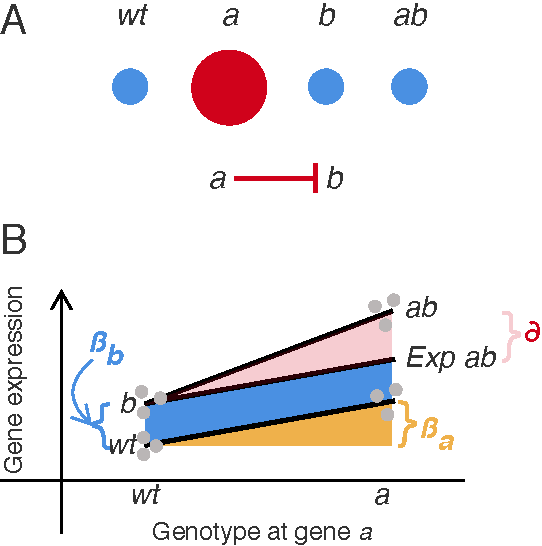
\includegraphics[width=\linewidth]{intro/epistasis.pdf}
  \caption{Biologists work with two distinct types of epistasis.
  \textbf{A}. Batesonian, or classical, epistasis refers to those cases where
  the qualitative phenotype associated with one null mutation is masked
  completely by the presence of a second mutation at a distinct locus.
  \textbf{B}. Generalized epistasis is used for quantitative phenotypes and
  measures the systematic deviation in the phenotype of a double mutant relative
  to a statistical null model. Unlike Batesonian epistasis, generalized
  epistasis cannot be used to infer genetic pathways, since the choice of null
  model is arbitrary. The effects associated with allele \(x\) are labelled
  \(\beta_x\), and the generalized epistasis is given the symbol \(\Delta \).
  }\label{fig:epistasis_example}
\end{figure}

Classical epistasis means that the phenotype of the double mutant is exactly the
same as the phenotype of one of the single mutants. However, the problem can
also be recast in quantitative terms. Statistical geneticists defined
generalized epistasis as a systematic deviation between the observed values and
a null model (usually additive or log-additive) that can be corrected by adding
a second order interaction term~\citep{Fisher1919}. In the terms of generalized
genetics, epistasis in the heterozygote crosses is measured in the systematic
excess of one phenotypic class and the systematic depletion of a second class.
Notably, generalized epistasis is not constrained in the values it can take, and
it is not constrained to measurements of population properties or properties of
single individuals.

As a result of its definition, the magnitude of generalized epistasis is
completely dependent on the null model selected by the researcher. Unlike
physical models that can be derived from first principles, statistical models of
genetic interactions are heuristic models that may or may not represent the
molecular interactions underlying the system accurately. In this sense, second
order `interaction' terms are \emph{ad hoc} corrections, technically
useful for machine-learning, but not instructive in terms of understanding the
genetic mechanisms at play. The conceptual proof for this is simple: Imagine
two different statistical models that describe how two genes interact along a
phenotype. Both models perform equally well. One of the models has a
statistically significant interaction (generalized epistasis) term whereas the
other does not. It is not possible to select one model over the other based on
statistical properties. In fact, based on model simplicity, we may even prefer
the model with fewer parameters, which could rule out the model that includes an
epistasis term.

Like classical epistasis, generalized epistasis has become a useful concept in
many areas of biology. Unlike classical epistasis, generalized epistasis
measurements have not been restricted to those generated by null alleles;
instead, generalized epistasis, particularly in human genetics, is measured
between any two molecular variants at different loci measured under a specific
null model. As a result of the subtle differences between classical and
generalized epistasis, there has been considerable concern about the apparent
disagreement between these two
concepts~\citep{Phillips2008,Cordell2002,Lehner2011}. In this review, we will
show how generalized and classical epistasis can be successfully unified.
Moreover, this unification has important ramifications for our ability to detect
genetic interactions between two mutants using in genome-wide studies.

\section*{Motivation: A brief introduction to RNA-sequencing}
RNA-sequencing~\citep{Mortazavi2008} is a powerful method that can measure all
the gene expression levels in an organism simultaneously. These measurements can
be made in bulk, from homogenized tissues or even from whole-organisms.
Recent technological breakthroughs have made measuring expression levels from
single whole organisms~\citep{Serra2018,Chan2018,Lott2011} or even single cells
possible~\citep{Tang2009}. As a result of its technical advantages, RNA-seq has
largely replaced microarrays as the method of choice to monitor gene expression.

Since the advent of genome-wide measurement methods, the idea of a cell- or
organismal-state, defined by its gene expression levels, has drawn significant
attention. Such states make sense in light of gene regulatory network theory,
which posits that the expression of many genes is coordinated by regulatory
factors that, when expressed, drive development forward~\citep{Britten1969}. A
common experimental design used to identify the genes that are controlled by a
specific regulatory module is to measure a baseline (typically wild type) sample
and a contrast sample where the regulatory module has been perturbed (often
through mutation). These experimental designs identify differentially expressed
genes between the wild type and the mutant samples. These batteries can then be
analyzed through ontological enrichment analyses that attempt to integrate
information from all the enriched transcripts and identify the biological
processes or signaling pathways contained within this list (see for
example~\citet{Mi2009,Angeles-Albores2016}). In spite of the enormous amount of
quantitative information that RNA-seq can provide about the genes that respond
to a downstream perturbation, these single factor experimental designs are
generally used to select a small number of novel downstream genes that can be
studied to extend a pathway of interest. The problem of how to analyze the rich
datasets generated by RNA-seq has proved difficult, and no one answer will be
suitable for all problems. Analyses of these datasets rely on a combination of
biological intuition, enrichment analyses or comparisons to other existing
datasets.

If we are willing to sacrifice the requirement for interpretability, these
datasets are still useful. Their practicality derives significantly from
enormous advances in library preparation methods~\citep{Picelli2014} and
improved quantification algorithms~\citep{Patro2014,Patro2015,Bray2016} that
have made RNA-seq an eminently replicable protocol that is fast to execute. As a
result, transcriptomes can readily be used to compare the extent to which two
perturbations are similar through clustering methods. Thus, transcriptomes could
be thought of as extremely long barcodes that are associated with specific,
potentially hidden, variables. If two barcodes are similar, then it is plausible
to hypothesize that the perturbations applied to generate each barcode were also
similar, even though we may not understand what these barcodes mean or how they
were generated. However, it is not sufficient to develop algorithms that show
two perturbations are similar on average. To use transcriptomes for genetic
analysis, we need methods that quantitatively reveal what aspects of two
transcriptomes are similar, by how much and that allow us to understand why they
are similar.

\section*{Genetic interactions detection through sequencing}
\subsection*{A brief overview of the problem}
Expression profiles are vectors where each entry corresponds to the expression
level of a single transcript. Conceptually, each entry could be treated as an
independent continuous phenotypes. Since continuous phenotypes can be used to
detect statistical epistasis, we could fit a statistical model to explain the
expression level of this transcript in each genotype measured (wild type, single
and double mutants). This statistical model will fit two parameters, \(\beta_a\)
and \(\beta_b\), that explain the \emph{individual} effects of each null
mutation, and a third parameter, \(\Delta \), quantifies the extent to which
these individual effects do not add when both null mutations are present at
once (see Fig.~\ref{fig:epistasis_example}). Each parameter is associated with a
\(p\)-value. These models are generated for every measured transcript. The
generated \(p\)-values should then be adjusted for multiple comparisons (these
adjusted values are referred to as \(q\)-values), and parameters with
\(q\)-values below a pre-specified threshold (often 0.1) are considered
statistically different from zero.

As a result, each transcript is associated with six values: the three model
parameters and their corresponding \(q\) values. At this point, the complexity
of the problem is obvious: Even if each parameter only acquires one of three
values (-, 0, +), there are 27 possible parameter combinations (epistatic
classes). Of these 27 classes, only four classes could give rise to the
classical epistasis regime (genetic suppression), so only those 4 classes can
give rise to a genetic diagram. One approach to visualize and attempt to
understand this complex space of epistatic combinations is to use heatmaps to
look for patterns and guide interpretation. This approach was used in
single-celled
organisms~\citep{Capaldi2008,VanDriessche2005,Sameith2015,VanDePeppel2005}, and
more recently has been used to perform high-throughput analyses of genetic
interactions in mammalian cells~\citep{Dixit2016}. Regression models with
interactions have also been successfully implemented using whole-organism
transcriptomic measurements~\citep{Angeles-Albores2017}.

The large number of parameter combinations is not the only (or major) drawback
to fitting models with interactions for every transcript. Another challenge is
the significant false positive and false negative rates for RNA-seq. RNA-seq
studies often accept an estimated false discovery rate of 10\%, and, although
false negative rates are unknown, estimates are as high as 90\% for mammalian
cells~\citep{Pimentel2016a}. These rates seriously impair attempts to classify
transcripts into any one of the 27 possible classes. If parameters are
controlled at a rate of 10\%, then the probability that at least one of the
parameters in a dense class (classes where all 3 parameters are + or -, not 0)
has been falsely accepted is almost 27\%. Thus, almost one in three of the
transcripts categorized into one of the 8 possible dense epistatic classes (+++,
- - -, ++-, etc\ldots) is misclassified and instead belongs to one of the twelve
doublet epistatic classes (++0, 0- -, etc\ldots). The situation becomes
considerably worse once we consider false negative rates, which are generally
unknown but estimates range up to 90\% in mammalian
systems~\citep{Pimentel2016a}. In general, false rates greatly exacerbate the
difficulties associated with analyzing transcriptomic datasets. If all
transcripts actually belonged to a single epistasis class to begin with, the
addition of statistical noise will split this class into many more classes that
mimicry complex interactions. The situation is further worsened by the fact that
interaction parameters can often be harder to measure than first order
parameters. Classifying transcripts into epistatic classes is a major obstacle
for successful epistatic analyses, and so far there has been little to no work
done to assess which classes are real and which are artifactual (some work has
been done in the context of allelic series, see
page~\pageref{sec:dominance_rev}). Equally concerning is the fact that none of
these epistatic classes can be translated into genetic diagrams. These epistatic
classes do not provide a biological mechanism (genetic, biochemical or cellular)
between the genes under study (see Fig.~\ref{fig:stat_methods}).

\begin{figure*}
  \centering{}
  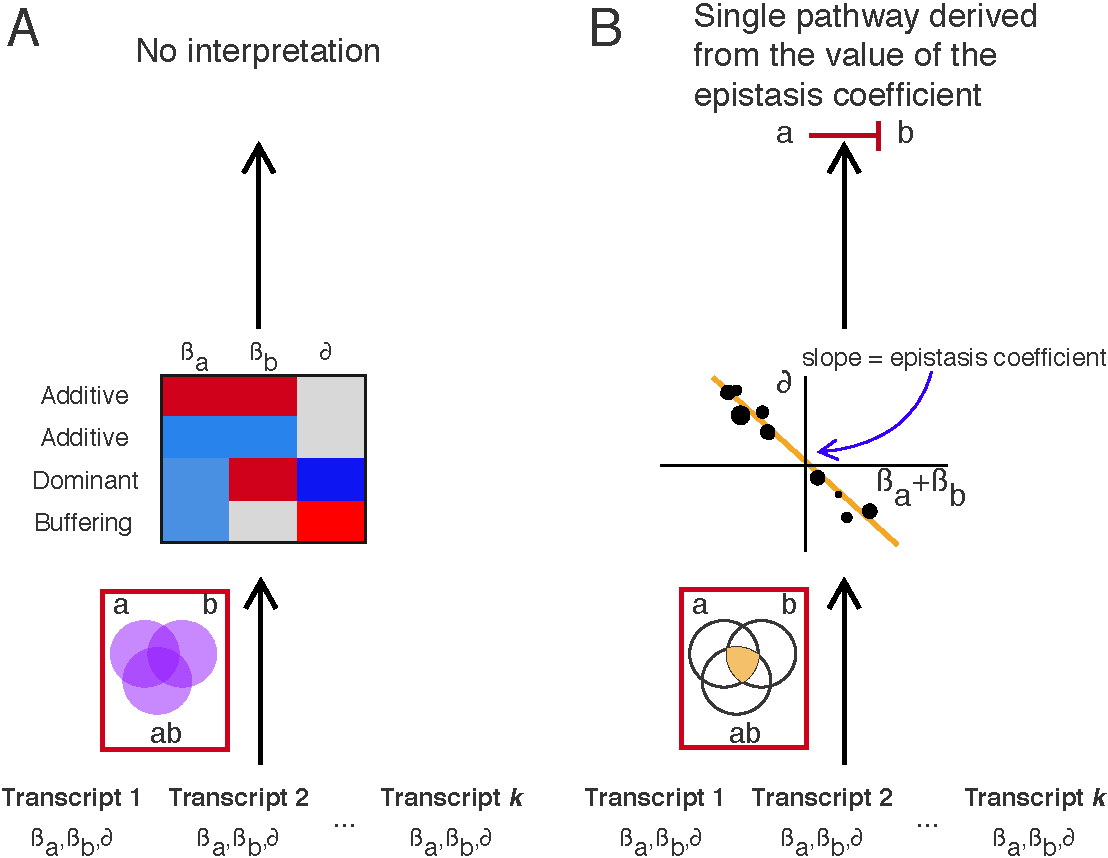
\includegraphics[width=.75\linewidth]{intro/epi_methods.pdf}
  \caption{Analysis methodology to infer genetic interactions using
  transcriptome data.
  \textbf{A}. After fitting all transcripts to a general linear model to
  calculate the individual and the epistatic components of null mutations in two
  distinct genes, the resulting parameters can be clustered and visualized in a
  heatmap. Each observed cluster can be grouped into one of 27 epistatic
  classes. All clusters are considered biologically relevant regardless of the
  number of transcripts they contain. A simple conclusion cannot be reached
  from these heatmaps. This approach was used in~\citet{Dixit2016} and~\citet{Adamson2016}
  \textbf{B}. Starting from the same statistical model, only transcripts that
  have all parameters different from zero are considered informative. These
  transcripts are plotted on a scatterplot, where the x-axis reflects the
  expected value of the double mutant under an additive or log-additive
  hypothesis, and the systematic deviation from additivity
  (generalized epistasis) is plotted on the y-axis. The resulting points form
  a ray on the plot. The slope of this ray is an aggregate statistic that can be
  interpreted in terms of a genetic pathway if the two genes exhibit Batesonian
  epistasis. This approach was used
  in~\citet{Angeles-Albores2017,Angeles-Albores2018a}}\label{fig:stat_methods}
\end{figure*}

\subsection*{Occam's razor, information pooling and constrained epistasis}
To extract biological mechanisms from transcriptome data, we must apply
simplifying constraints. If transcripts are to be classified into 27 possible
epistatic classes, we must develop methods to assess which of these classes have
sufficient statistical leverage to accept their existence (in other words, we
need a statistical test that examines the null hypothesis that such a class
could appear purely by chance). However, even if such a test were developed, we
still require a method that allows us to summarize the information in these
modules, and which lets us build a genetic pathway if the data suggests a
pathway exists. A natural way to do this may be to use the natural structure of
biological networks to pool the information from all transcripts, and test the
interaction of this \emph{structure} between the two mutants, instead of testing
the individual transcripts. Information sharing is a powerful concept that
allows us to incorporate more data points into a calculation, thus increasing
our statistical power for any single test, but it requires the data to be drawn
from a structure that permits sharing.

One such information sharing approach was implemented
in~\citet{Angeles-Albores2018a,Angeles-Albores2017}. Briefly, these studies
obtained whole-organism bulk RNA-seq transcriptome profiles for single and
double perturbations and identified differentially expressed transcripts in each
condition relative to the wild-type. Next, transcripts that were differentially
expressed in all non-control conditions were aggregated and analyzed jointly for
systematic deviations from a linear pathway. This systematic deviation was
quantified in a single coefficient, called the transcriptome-wide epistasis
coefficient. This coefficient can be interpreted in terms of simple genetic
pathways because it can be used to test whether the perturbations result in a
phenotypic transformation diagnostic of Batesonian epistasis. In this sense, the
transcriptome-wide epistasis coefficient represents a unification of generalized
epistasis and classical epistasis. This approach is powerful because it avoids
multiple hypothesis testing (a single interaction coefficient is tested), and it
doesn't rely on any one transcript to draw conclusions. A significant advantage
of this method is that these studies were able to test and verify that the
generalized epistasis measurements they made were equivalent to Batesonian
epistasis (in other words, the double mutant had the same perturbations as one
of the single mutants), culminating in a formal genetic pathway. Both studies
assumed that the genetic interaction between two genes is unimodal, in other
words, these two genes do not interact along multiple pathways with different
strengths and valences. This last assumption may not always hold. This strongly
simplifying assumption contrasts with the previously referenced work that
assumes unbounded complexity for all genetic interactions. Neither is correct,
though it is our opinion that biological interactions tend to be much simpler
than is often assumed in genomic studies.

\section*{Beyond genetic interactions: Dominance studies to map gene
          functions}\label{sec:dominance_rev}
Although transcriptomes have been used as phenotypes for analysis of genetic
interactions for many years, their uses need not be restricted for theoretic
analysis. In population genetics, transcriptomes have been used as phenotypes
with which to identify expression quantitative trait loci in a number of
organisms~\citep{Brem2002,DeCook2006,Kirst2004,Schadt2003}. Transcriptomes can
also be used to compare the genetical properties of different alleles of a
single gene~\citep{Angeles-Albores2018b}.

Allelic series require considerably more analysis than tests for genetic
interactions. To infer functional units from the activity of multiple allelic
variants, the phenotypes associated with each variant must be carefully
enumerated. Alleles must be ordered according to the phenotypic severity they
cause when animals are homozygotes for each variant, with a separate hierarchy
drawn for each phenotype. Alleles must also be ordered according to their
dominance hierarchy over other alleles along each phenotype by measured the
phenotypes of \emph{trans}-heterozygotes. Particular care must be taken to
ensure that the phenotypes of the \emph{trans}-heterozygotes are not the result
of maternal effects by testing progeny generated from a second, reciprocal,
cross. The overall results are examined and the most parsimonious explanation is
accepted to draw functional units and establish their sequence requirements. The
the number and resolution of the functional units that can be defined depends on
the density of the allelic series that is tested. For a more thorough
introduction to dominance and its role in allelic series, see~\citet{Yook2005}.

As a result of the rigor required to analyze them, allelic series provides an
excellent testing ground in which to explore the potential, but also the
shortcomings, of transcriptomes as molecular phenotypes. To be successful, the
analysis of even the smallest allelic series must order the tested variants.
\citet{Angeles-Albores2018b} reported the first allelic series, to our
knowledge, to be analyzed using expression profiles in any organism. In this
analysis, the transcriptomic analogue of distinct phenotypes, phenotypic classes
consisting of groups of differentially expressed genes, were identified by
labelling each gene with the genotypes where it was differentially expressed.
Subsequently, the expression level of these genes in \emph{trans}-heterozygotes
was approximated by a linear combination of the expression levels in each
homozygote, with the weighting coefficients constrained to add to unity. The
weighting coefficients, bounded in this manner, reflect the dominance of one
allele over the other. These transcriptome-wide dominance coefficients are
analogous to the transcriptome-wide epistasis aggregate statistics derived in
previous studies~\citep{Angeles-Albores2018a}. The intersections from the Venn
diagram (see Fig.~\ref{fig:dominance_expl}) are understood to occur as a result
of the activity of one or more functional units which may or may not have
dosage-saturated activity (this is inferred from the dominance behavior of
the given intersection).

\begin{figure}
  \centering
  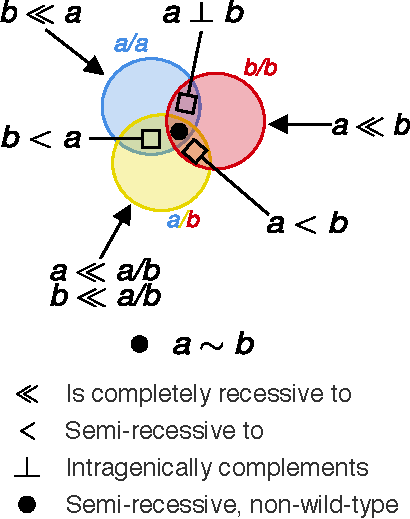
\includegraphics{intro/dominance.pdf}
  \caption{Genes that are differentially expressed in genotypes containing
  mutant (\allele{a}, \allele{b}) alleles relative to a wild type homozygote can
  be categorized into phenotypic classes. Each phenotypic class can in turn be
  associated with a dominance behavior. The Venn diagram represents
  differentially expressed transcripts in each genotype relative to the
  wild-type control. Each of the possible 7 intersections is labelled with its
  dominance interpretation if the intersection is real. In this context,
  semi-recessiveness means that one allele is partially or completely dominant
  to the other along a continuous spectrum between 0 and 1. The dominance sign
  between an allele and the heterozygote genotype indicates heterosis or
  over-dominance.}\label{fig:dominance_expl}
\end{figure}

This study highlighted the importance of recognizing and characterizing the
statistical artifacts that can occur in genomic datasets (see
Fig.~\ref{fig:noisy_venn}). The analyzed dataset had sufficiently large false
positive and false negative rates to generate artificial phenotypic classes that
nevertheless could be identified and removed from the analysis. Unlike epistatic
classes, for which we do not have a sense of what classes can most easily arise
as a result of statistical artifacts, all the phenotypic classes arising from
allelic series analyses can be readily interpreted in terms of inter-allelic
complementation, a phenomenon that is extremely well characterized in genetics.
Allelic series provide an excellent testing ground in which to explore
algorithms to partition transcriptomes into gene batteries that have sufficient
statistical support, since it is possible to have an intuition for artifactual
classes.

\begin{figure}
  \centering
  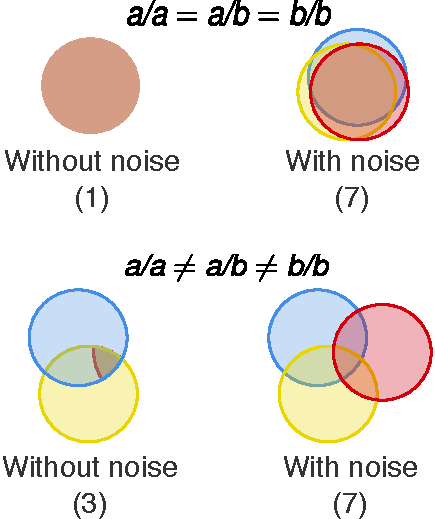
\includegraphics{intro/noisy_venn.pdf}
  \caption{RNA-seq artifacts can greatly exaggerate apparent biological
  complexity. We considered the case where we have two phenotypically identical
  alleles that can be used to generate the genotypes \genotype{a/a},
  \genotype{b/b} and \genotype{a/b}. In the absence of artifacts, the set of
  differentially expressed transcripts relative to a wild-type control should be
  the same amongst all three genotypes. However, if measurement error occurs,
  then instead of observing a single Venn intersection, we will observe seven
  intersections. If these intersections are not identified as false, we would
  wrongly conclude that allele \allele{a} and \allele{b} are not phenotypically
  equivalent, incurring in an error rate of 600\%. Even in the case where
  the three genotypes are not equivalent, statistical noise will tend to
  significantly increase the apparent biological complexity present in the
  system (from 3 to 7 in this example). In general, statistical artifacts are so
  common in genomic assays that they will tend to generate all the possible
  intersections in a comparison. This highlights the need to apply simplifying
  constraints on transcriptome data before interpreting the
  results.}\label{fig:noisy_venn}
\end{figure}


\section*{Open problems and opportunities}
RNA-sequencing is becoming increasingly easier and cheaper. RNA-seq offers a
powerful, unbiased approach to genetics that can be multiplexed in many systems
relatively easily. We expect that genetics using expression profiles will be an
excellent first-pass assay because of the speed and sheer amount of information
associated with the generation of expression profiles. These properties make
RNA-seq particularly advantageous for groups that are studying relatively
unknown genes or genes with subtle phenotypes. RNA-seq may also be a powerful
method to complement genetics in emerging model organisms where conventional
genetics may be laborious and where researchers may wish to minimize the number
of experiments performed while maximizing the amount they can learn.

A major challenge moving forward will be mixed epistasis analyses with allelic
series. Such mixed analyses try to identify the sequence requirements of one
gene to participate in an epistatic interaction, and to test whether the
observed epistatic interaction between two genes reflects a single biochemical
function or the joint activity of distinct molecular properties. For example, in
\cel{} the inhibition of \gene{hif-1} by \gene{egl-9} is mediated partially by
the hydroxylation of HIF-1 by EGL-9, and partially through a
hydroxylation-independent mechanism that is not well
understood~\citep{Shao2009}. The high false positive and false negative rates
inherent to RNA-seq means that all interactions amongst all genes will appear to
be the compounded result of many independent activities. The solution to this
problem will require methods that can incorporate information not just between
single and double mutants, or homozygotes and heterozygotes, but amongst
epistatic modules and dominance modules while searching for the most
parsimonious structure that can explain all the expression profiles.

A second challenge will be the association of gene batteries with other
observable phenotypes to develop signatures that allow us to read and interpret
a transcriptome in terms of biological covariates. In other words, we would like
signatures that allowed us to infer what the organism was doing when the RNA
was extracted, what pathways had been disrupted or activated, what cellular or
morphological phenotypes it exhibited. Such signatures could be derived by
allowing organisms to undergo a specific life history, then extracting the
transcriptome and associating the differentially expressed genes in response to
this life history relative to a control history to derive a signature.
Alternatively, single-cell or single-organism methods may be able to track
organisms, recording their behavior, before extracting their
RNA~\citep{Lane2017}. These signatures, although useful, should not be treated
as causal, because the derivation of these signatures is through correlation.
Deriving causal signatures would be very interesting and potentially useful as
well, since this would make the discovery and association of novel pathways
considerably easier. A significant weakness of expression signatures is that
they only make sense relative to a baseline control, and therefore signatures
can only be associated with events that have a sufficient dynamic range relative
to the baseline. Another problem with signatures is the arbitrary definition,
since they will inevitably be defined according to a \(q\)-value cut-off.
It seems reasonable to postulate that eventually we must abandon the concept of
differential expression: It is too brittle, too relativistic and prevents us
from thinking about the transcriptome as a complete object.

Without transcriptional signatures of some sort, understanding modules will be
all but impossible. Even with signatures, modules will be explained only
phenomenologically: We know this signature is correlated to this phenotype,
therefore this module is correlated to the same phenotype. With time, we may be
able to understand mechanistically why specific phenotypes are correlated with
the expression of specific genes. For the moment, such understanding seems far
from our reach.

In the end, the major challenge for transcriptome genetics is likely to be our
own creativity. New phenotypes always have their difficulties and drawbacks, and
expression profiles are no exception. Expression profiles will not, on their
own, reconstruct every network or solve all of biology. However, expression
profiles are an object of a new kind, with behaviors that we do not fully
understand hiding novel biological phenomena. It has become evident that
genetics is applicable at an enormous range of phenotypes, from population
phenotypes to organismal to macroscopic and mesoscopic phenotypes.
Transcriptomes represent a new phenotype at the microscopic and genomic level.
Perhaps surprisingly, these microscopic phenotypes, in spite of all their
complexity, seem to obey the genetic properties that bind all other phenotypes.
The challenge, then, is how to use transcriptomes to discover biological
principles that help us understand how the hierarchy of cells, organs, organisms
and populations emerges from the collective actions of a string of atoms.
